\chapter{Массы фермионов: хиральность, юкавские взаимодействия и нейтрино Майораны}

\lectureoverview{Сначала мы заново строим хиггсовский механизм для калибровочных бозонов в игрушечной \(U(1)\)-теории, а затем задаём параллельный вопрос о фермионах. Дираковский массовый член смешивает поля левой и правой хиральности, однако слабое взаимодействие приписывает им разные заряды и потому запрещает голый массовый член. Юкавское взаимодействие с полем Хиггса сохраняет симметрию; после того как поле Хиггса приобретает вакуумное значение, то же взаимодействие превращается в массу фермиона и в измеримое взаимодействие Хиггса--фермиона. В заключительной части эта логика переносится на массу нейтрино, возможные тяжёлые незащищённые частицы, кинематику космических лучей, релятивистскую инерцию и гравитацию.}

Цель вступительного повторения состоит не просто в том, чтобы повторить предыдущую лекцию. Нам нужна одна идея из неё в виде, который можно перенести на фермионы: масса — это ненулевая энергия возбуждения при нулевом импульсе. Для поля нулевой импульс означает бесконечную длину волны, или смещение, одинаковое всюду. Теория, содержащая только производные, не может обнаружить однородное смещение. Член без производных может.

\section{История калибровочных бозонов за один проход}

\subsection{Энергия, связанная с производными, и безмассовый вектор}

Модельное калибровочное поле — \(A_\mu\), а его тензор напряжённости равен
\begin{equation}
  F_{\mu\nu}
  =\partial_\mu A_\nu-\partial_\nu A_\mu .
  \label{eq:l09-field-strength}
\end{equation}
На доске кинетический член калибровочного поля схематически записан как \(F^2\). При стандартной нормировке он имеет вид
\begin{equation}
  \mathcal L_{\mathrm{gauge}}
  =-\frac14 F_{\mu\nu}F^{\mu\nu}.
  \label{eq:l09-gauge-kinetic}
\end{equation}

\begin{figure}[htbp]
\centering
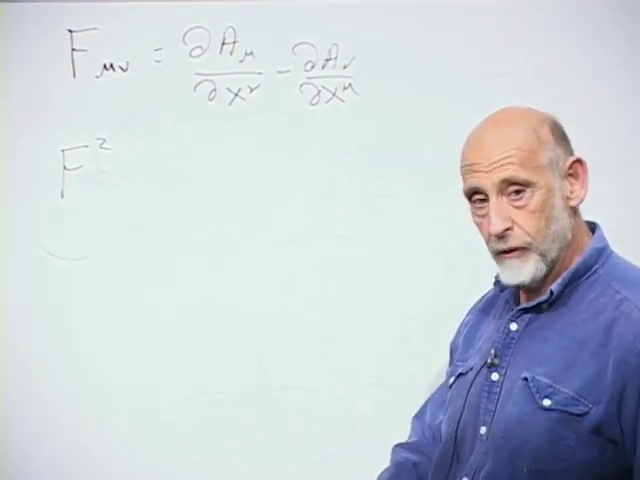
\includegraphics[width=0.72\textwidth]{lecture_09_figure_02.png}
\caption{Определение тензора напряжённости поля и используемое на доске сокращение \(F^2\) для энергии калибровочного поля, зависящей от производных.}
\lectureframe{00:02:39}
\label{fig:l09-field-strength-board}
\end{figure}

Каждое вхождение \(A_\mu\) в \eqref{eq:l09-gauge-kinetic} стоит под знаком производной. Следовательно,
\begin{equation}
  A_\mu(x)\longmapsto A_\mu(x)+c_\mu,
  \qquad \partial_\nu c_\mu=0,
\end{equation}
не изменяет \(F_{\mu\nu}\). Поэтому однородный векторный потенциал не требует энергии напряжённости поля. В терминах лекции мода с нулевым импульсом не имеет щели, и калибровочный бозон безмассов.

Это поле \(U(1)\) — намеренно простой заменитель. Физическая цель здесь — \(W^\pm\) и \(Z\), а не фотон электромагнитного взаимодействия. Ненарушенная электромагнитная симметрия оставляет фотон безмассовым; нарушенная электрослабая симметрия придаёт массы слабым калибровочным бозонам.

\subsection{Замораживание радиуса поля Хиггса}

Введём заряженное комплексное скалярное поле и запишем его в полярной форме:
\begin{equation}
  \phi(x)=\rho(x)e^{i\alpha(x)}.
\end{equation}
Его потенциал типа мексиканской шляпы минимален на окружности ненулевого радиуса. Обозначив этот радиус через \(f\), заметим, что радиальное направление сравнительно жёсткое. В первом рассмотрении мы заморозим его и оставим только фазу:
\begin{equation}
  \phi(x)\simeq f e^{i\alpha(x)}.
  \label{eq:l09-frozen-higgs}
\end{equation}

\begin{figure}[htbp]
\centering
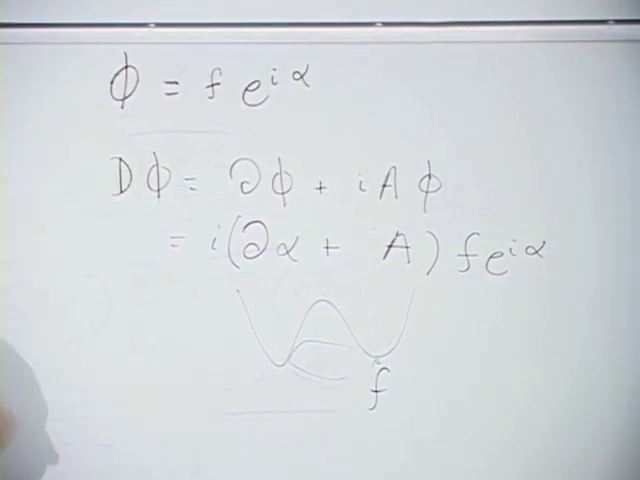
\includegraphics[width=0.72\textwidth]{lecture_09_figure_03.png}
\caption{Замороженный радиус поля Хиггса, его ковариантная производная и маленький эскиз нарушенного потенциала, использованный в повторении.}
\lectureframe{00:06:42}
\label{fig:l09-frozen-board}
\end{figure}

Выберем соглашение
\begin{equation}
\begin{aligned}
  D_\mu&=\partial_\mu+igA_\mu,
  \\
  \phi&\longmapsto e^{i\theta}\phi,
  \\
  A_\mu&\longmapsto A_\mu-\frac1g\partial_\mu\theta .
\end{aligned}
  \label{eq:l09-gauge-convention}
\end{equation}
В лекции \(g\) опускается; если оставить его явно, размерности и итоговая масса становятся ясными. Действуя на замороженное поле, получаем
\begin{align}
  D_\mu\phi
  &=(\partial_\mu+igA_\mu)f e^{i\alpha}
  \notag\\
  &=i\bigl(\partial_\mu\alpha+gA_\mu\bigr)
    f e^{i\alpha}.
  \label{eq:l09-covariant-frozen}
\end{align}
Умножение на комплексно-сопряжённое убирает фазу и одновременно превращает \(i\), умноженное на \(-i\), в \(+1\):
\begin{equation}
  |D_\mu\phi|^2
  =f^2
   \bigl(\partial_\mu\alpha+gA_\mu\bigr)
   \bigl(\partial^\mu\alpha+gA^\mu\bigr).
  \label{eq:l09-frozen-square}
\end{equation}

\begin{classroomqa}
\audiencequestion{Должен ли квадрат ковариантной производной содержать минус, потому что производная дала множитель \(i\)?
\lecturetimestamp{00:07:39}}
\lecturerresponse{Нет. Кинетический член — это произведение с комплексно-сопряжённым. Один множитель даёт \(i\), другой \(-i\), и \(i(-i)=1\). Соглашение о знаке в \(D_\mu\) можно последовательно обратить, но квадрат модуля в соответствующем выражении для энергии остаётся положительным.}
\end{classroomqa}

Комбинация в \eqref{eq:l09-frozen-square} сама является сдвинутым калибровочным полем. Выберем \(\theta=-\alpha\), чтобы фаза скаляра исчезла, и определим
\begin{equation}
  A'_\mu=A_\mu+\frac1g\partial_\mu\alpha .
  \label{eq:l09-unitary-gauge-field}
\end{equation}
Тогда
\begin{equation}
  |D_\mu\phi|^2=g^2f^2 A'_\mu A'^\mu .
  \label{eq:l09-vector-mass-term}
\end{equation}
Новый член не содержит производной от \(A'_\mu\). Однородное поле теперь запасает энергию, так что векторная мода при нулевом импульсе имеет щель.

\begin{figure}[htbp]
\centering
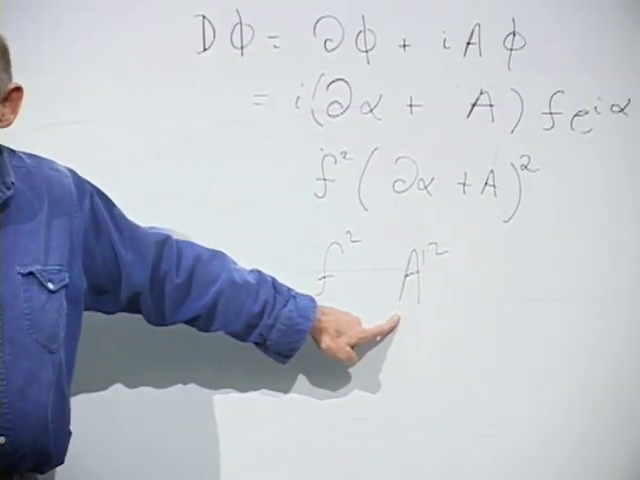
\includegraphics[width=0.72\textwidth]{lecture_09_figure_04.png}
\caption{На доске выделен член \(f^2A^2\), указывающий на массу калибровочного бозона после поглощения фазы.}
\lectureframe{00:10:31}
\label{fig:l09-vector-mass-board}
\end{figure}

При канонической нормировке скаляра пишут
\(\phi=(f+h)e^{i\pi/f}/\sqrt2\). Сравнение возникающего векторного члена с
\(\tfrac12m_A^2A_\mu A^\mu\) даёт
\begin{equation}
  m_A=gf
  \label{eq:l09-abelian-vector-mass}
\end{equation}
в этой абелевой модели. В лекции множители нормировки опускаются, и результат суммируется утверждением, что масса векторного бозона задаётся величиной \(f\).

Фазовая мода не исчезла бесследно. До введения калибровочного поля она была безмассовым бозоном Голдстоуна. После калибровки она обеспечивает продольную поляризацию, необходимую массивной векторной частице. Радиальное возбуждение, которое мы временно заморозили, остаётся физическим хиггсовским возбуждением.

\subsection{Почему член без производных означает массу}

\begin{classroomqa}
\audiencequestion{Почему член \(A'^2\) считается массовым членом, а не просто ещё одним взаимодействием?\lecturetimestamp{00:13:10}}
\lecturerresponse{Масса — это энергия в покое. Для поля частица в покое есть квант моды с нулевым импульсом и бесконечной длиной волны. Член с производными не даёт энергии статическому однородному смещению, тогда как \(m_A^2A'^2\) даёт. Эта ненулевая энергия при нулевом импульсе и есть щель по энергии покоя.}
\end{classroomqa}

Лекция развивает это утверждение через три механические аналогии.

\begin{itemize}
  \item В кристалле медленно меняющееся смещение требует упругой энергии, потому что соседние атомы смещаются по-разному. Жёсткий перенос сдвигает все атомы вместе и не требует внутренней энергии. Поэтому акустический фонон не имеет щели.
  \item В идеальном магните с вращательной симметрией пространственно меняющееся направление спина требует обменной энергии, но совместный поворот всех спинов — нет. Поэтому соответствующая длинноволновая спиновая волна не имеет щели.
  \item В плазме смещение электронной жидкости относительно положительного фона создаёт разделение зарядов и восстанавливающее электрическое поле даже при однородном относительном смещении. Поэтому плазмон имеет ненулевую частоту при нулевом волновом числе.
\end{itemize}

Калибровочное поле после механизма Хиггса ведёт себя как в третьем примере: среда с нарушенной симметрией сопротивляется тому, что иначе было бы однородным смещением без энергетической цены.

\begin{classroomqa}
\audiencequestion{До введения калибровочного поля разве фаза \(\alpha\) уже не колебалась?\lecturetimestamp{00:18:24}}
\lecturerresponse{Колебалась. Её энергия была пропорциональна \(f^2(\partial_\mu\alpha)^2\). Фаза, меняющаяся от точки к точке, имеет градиентную энергию и может распространяться, но однородное изменение фазы ничего не стоит. Это и есть безмассовая голдстоуновская мода.}
\end{classroomqa}

\begin{classroomqa}
\audiencequestion{Производная включает и производную по времени. Разве реальное перемещение всей решётки или изменение всего поля не несёт кинетической энергии?\lecturetimestamp{00:22:18}}
\lecturerresponse{Да. Сравнение проводится между статическими конфигурациями или между конфигурациями, подготовленными сколь угодно медленно. Решётка, движущаяся с ненулевой скоростью, имеет кинетическую энергию. Проверка на массу спрашивает, остаётся ли у конфигурации энергия, когда она покоится и пространственно однородна.}
\end{classroomqa}

\section{Экспериментальная подсказка: слабые взаимодействия различают левое и правое}

Теперь лекция переходит к электрону, мюону и кваркам. Их массы тоже возникают из поля Хиггса, но механизм выглядит иначе, потому что масса фермиона — это не квадратичный векторный член. Это связь между двумя хиральными полями.

\subsection{Нарушение чётности в бета-распаде}

Начнём с эмпирического факта: слабое взаимодействие нарушает чётность. Квантовая электродинамика и квантовая хромодинамика одинаково относятся к процессу и его зеркальному отражению. Слабое взаимодействие — нет. В бета-распаде нейтрона,
\begin{equation}
  n\longrightarrow p+e^-+\bar\nu_e,
  \label{eq:l09-beta-decay}
\end{equation}
высокоэнергетические электроны, отобранные взаимодействием заряженного тока, обладают левой спиральностью: их спин направлен противоположно импульсу. Соответствующие антинейтрино имеют противоположную спиральность.

Для ультрарелятивистской частицы определим спиральность как
\begin{equation}
  h=\frac{\bm S\cdot\bm p}{|\bm S|\,|\bm p|}.
\end{equation}
Спин, параллельный импульсу, имеет \(h=+1\); антипараллельный — \(h=-1\). Слабое взаимодействие связывается с левохиральным электронным полем и левохиральным нейтринным полем, но не с правохиральным электронным полем таким же образом.\editorialnote{Сначала в лекции используется лево- и праворукость в смысле спиральности, потому что при высоких энергиях это наглядно. Калибровочные заряды на самом деле действуют на хиральность — метку представления группы Лоренца, выделяемую \(P_L=(1-\gamma^5)/2\) и \(P_R=(1+\gamma^5)/2\). Для безмассовой частицы хиральность и спиральность у частиц совпадают; для массивной частицы — нет.}

Чтобы увидеть это препятствие, не вводя полный аппарат \(SU(2)_L\times U(1)_Y\), вообразим фиктивный мир \(U(1)\), в котором соответствующий заряд несёт только \(\psi_L\):
\begin{equation}
  \psi_L\longmapsto e^{i\theta}\psi_L,
  \qquad
  \psi_R\longmapsto\psi_R .
  \label{eq:l09-chiral-toy-charge}
\end{equation}
Это не электромагнетизм: реальные лево- и правохиральные электроны несут один и тот же электрический заряд. Это карикатура на слабое взаимодействие, в котором две хиральности находятся в разных электрослабых представлениях.

\begin{classroomqa}
\audiencequestion{Применима ли та же лево--правая асимметрия к кваркам?
\lecturetimestamp{00:31:50}}
\lecturerresponse{Да, при соответствующих слабых мультиплетах и гиперзарядах. Левохиральные кварки верхнего и нижнего типов образуют слабые дублеты, тогда как правохиральные поля являются слабыми синглетами. Поэтому их связи с полем Хиггса сталкиваются с той же структурной проблемой, что и у электрона.}
\end{classroomqa}

\section{Масса Дирака — это лево--правое смешивание}

\subsection{От четырёхкомпонентного уравнения к двум уравнениям Вейля}

Дираковская волновая функция имеет четыре компоненты. Грубо говоря, две из них описывают спин, а две различают решения с положительной и отрицательной энергией, причём последние переинтерпретируются как степени свободы античастицы. В гамильтоновой форме,
\begin{equation}
  i\frac{\partial\Psi}{\partial t}
  =\left(-i\bm\alpha\cdot\bm\nabla+m\beta\right)\Psi .
  \label{eq:l09-dirac-hamiltonian}
\end{equation}
Матрицы \(\alpha_i\) и \(\beta\) кодируют релятивистскую связь между энергией, импульсом и массой.

\begin{figure}[htbp]
\centering
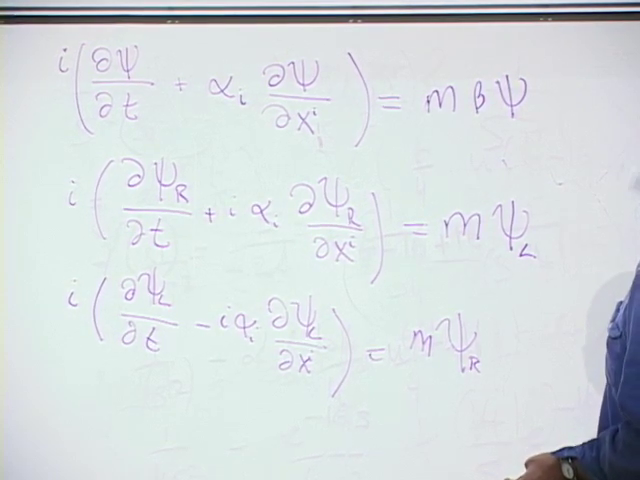
\includegraphics[width=0.74\textwidth]{lecture_09_figure_05.png}
\caption{Сначала на доске записывается уравнение Дирака, а затем оно разлагается на связанные уравнения для левохиральной и правохиральной компонент.}
\lectureframe{00:40:30}
\label{fig:l09-dirac-board}
\end{figure}

Хиральный базис делает роль \(m\) явной. При \(\sigma^\mu=(1,\bm\sigma)\) и \(\bar\sigma^\mu=(1,-\bm\sigma)\),
\begin{align}
  i\bar\sigma^\mu\partial_\mu\psi_L&=m\psi_R,
  \label{eq:l09-weyl-left}\\
  i\sigma^\mu\partial_\mu\psi_R&=m\psi_L.
  \label{eq:l09-weyl-right}
\end{align}
При \(m=0\) уравнения независимы: левохиральное поле и правохиральное поле могут распространяться, не взаимодействуя друг с другом. При \(m\neq0\) каждое из них выступает источником для другого. Именно в этом точном смысле масса Дирака смешивает левое и правое.

Сасскинд описывает это как осцилляции фермиона между левым и правым состояниями. Такая формулировка передаёт связь, но её не следует превращать в буквальную классическую картину точечной частицы, переворачивающейся туда-сюда. Точное утверждение — система связанных полевых уравнений
\eqref{eq:l09-weyl-left}--\eqref{eq:l09-weyl-right}.

\begin{classroomqa}
\audiencequestion{Согласованы ли множители \(i\) и знаки в двух уравнениях на доске?\lecturetimestamp{00:41:10}}
\lecturerresponse{Не построчно на доске; при быстром выводе один \(i\) был непоследовательно вынесен наружу. Надёжное содержание здесь — структура связи. Уравнения \eqref{eq:l09-weyl-left} и \eqref{eq:l09-weyl-right} задают одну стандартную согласованную конвенцию.}
\end{classroomqa}

\subsection{Почему слабая симметрия запрещает голую массу}

Соответствующий массовый член Дирака в лагранжиане имеет вид
\begin{equation}
  \mathcal L_m
  =-m\bar\psi\psi
  =-m\left(\bar\psi_L\psi_R+\bar\psi_R\psi_L\right).
  \label{eq:l09-bare-dirac-mass}
\end{equation}
При упрощённом преобразовании \eqref{eq:l09-chiral-toy-charge},
\begin{equation}
  \bar\psi_L\psi_R\longmapsto
  e^{-i\theta}\bar\psi_L\psi_R,
  \qquad
  \bar\psi_R\psi_L\longmapsto
  e^{i\theta}\bar\psi_R\psi_L.
\end{equation}
Ни один из этих членов не инвариантен. Поэтому до нарушения симметрии коэффициент \(m\) прямого лево--правого смешивания запрещён.

Одно лишь электромагнитное взаимодействие не создало бы этой проблемы, поскольку \(\psi_L\) и \(\psi_R\) имеют одинаковый электрический заряд. Препятствие возникает из-за их разных слабых квантовых чисел.

\subsection{Вопросы о спиральности, выявляющие тонкость хиральности}

Теперь слушатели проверяют интуитивную картину левости и правости с нескольких сторон. Эти вопросы не побочны: они точно показывают, где спиральность полезна, а где её должна заменить хиральность.

\begin{classroomqa}
\audiencequestion{Каким был бы мир, если бы слабое взаимодействие испускало электроны обеих спиральностей с равной вероятностью?\lecturetimestamp{00:42:12}}
\lecturerresponse{Непосредственная асимметрия по чётности в этом процессе исчезла бы. Но реальная электрослабая теория хиральна: в заряжённом слабом взаимодействии участвуют только левохиральные дублеты. В лекции более полный разбор того, почему природа выбрала такую структуру, откладывается.}
\end{classroomqa}

\begin{classroomqa}
\audiencequestion{Предположим, спин электрона подготовлен вертикально, а затем электрон разгоняют горизонтально. Будет ли он лево- или правоспиральным?
\lecturetimestamp{00:42:44}}
\lecturerresponse{Состояние со спином, поперечным импульсу, является суперпозицией двух спиральностей. Спиральность определена точно только тогда, когда спин параллелен или антипараллелен импульсу. Тем не менее слабые хиральные проекторы для поля определены однозначно.}
\end{classroomqa}

Массивную частицу можно замедлить до покоя и затем разогнать в противоположном направлении, не обращая её спин. Тогда её спиральность меняет знак. Безмассовую частицу нельзя ни перегнать, ни привести в состояние покоя преобразованием Лоренца, поэтому её спиральность инвариантна относительно собственных бустов. Это мотивирует сформулированное в лекции утверждение, что частица данного вида, имеющая только одну физическую спиральность, должна быть безмассовой. Более точное утверждение теории поля состоит в том, что лоренц-инвариантная масса Дирака требует обеих хиральностей.

\begin{classroomqa}
\audiencequestion{Фотон с круговой поляризацией может отразиться от зеркала и изменить направление на противоположное, ни на мгновение не переходя в состояние покоя. Не противоречит ли это аргументу о спиральности?\lecturetimestamp{00:45:28}}
\lecturerresponse{Нет. Зеркало — внешняя система, способная обмениваться угловым моментом и обращать направление распространения. Процесс отражения не является лоренцевым бустом, который перегоняет фотон. Возможность существования канала зависит также от допустимых состояний поляризации и от граничных условий на поверхности материала.}
\end{classroomqa}

\begin{classroomqa}
\audiencequestion{Содержит ли обычный электронный пучок частицы только одной спиральности или обеих?\lecturetimestamp{00:46:10}}
\lecturerresponse{Вообще говоря, обеих. Состояние массивного электрона содержит обе хиральные компоненты, а неполяризованный пучок содержит обе спиральности. Специализированные источники могут создавать поляризованный пучок с большой асимметрией по спиральности.}
\end{classroomqa}

\begin{classroomqa}
\audiencequestion{Можно ли сфокусировать пучок независимо от его спина, или магнитные поля разделяют две поляризации?\lecturetimestamp{00:46:29}}
\lecturerresponse{Обычная пространственная фокусировка может быть в значительной степени нечувствительной к спину, но магнитные моменты взаимодействуют с градиентами магнитного поля. Поэтому спин-селективные источники, градиенты типа Штерна--Герлаха и спиновая динамика в ускорителях могут подготавливать или разделять поляризации.}
\end{classroomqa}

\begin{classroomqa}
\audiencequestion{Является ли слабое различие между левым и правым всего лишь случайностью?\lecturetimestamp{00:48:13}}
\lecturerresponse{В рамках данного курса это экспериментальный факт, заложенный в Стандартную модель. Он слишком систематичен, чтобы выглядеть простым случайным совпадением, но сама Стандартная модель не выводит полный набор хиральных зарядов из более глубокого принципа.}
\end{classroomqa}

\section{Юкавская конструкция}

\subsection{Пусть Хиггс несёт недостающий заряд}

Симметрия запрещает массовый параметр в виде числа, но допускает взаимодействие с полем, которое даёт недостающую фазу преобразования. Введём комплексный скаляр с
\begin{equation}
  \phi\longmapsto e^{i\theta}\phi,
  \qquad
  \phi^\dagger\longmapsto e^{-i\theta}\phi^\dagger.
  \label{eq:l09-scalar-charge}
\end{equation}
Тогда
\begin{equation}
  \mathcal L_Y
  =-y\,\bar\psi_L\phi\psi_R
   -y^*\,\bar\psi_R\phi^\dagger\psi_L
  \label{eq:l09-yukawa-lagrangian}
\end{equation}
калибровочно инвариантно. В первом члене \(\bar\psi_L\) даёт множитель \(e^{-i\theta}\), а \(\phi\) даёт \(e^{i\theta}\); фазы сокращаются. Второй член является эрмитово-сопряжённым к первому.

Эквивалентно, хиральные уравнения приобретают зависящее от поля смешивание:
\begin{align}
  i\bar\sigma^\mu D_\mu\psi_L
    &=y\phi\psi_R,
  \label{eq:l09-yukawa-eom-left}\\
  i\sigma^\mu\partial_\mu\psi_R
    &=y^*\phi^\dagger\psi_L.
  \label{eq:l09-yukawa-eom-right}
\end{align}

\begin{figure}[htbp]
\centering
\includegraphics[width=0.76\textwidth]{lecture_09_figure_06.png}
\caption{Голая масса в правых частях заменена заряженным скалярным полем. Точные знаки на доске схематичны; инвариантная структура дана в \eqref{eq:l09-yukawa-lagrangian}.}
\lectureframe{00:51:30}
\label{fig:l09-yukawa-board}
\end{figure}

До нарушения симметрии это взаимодействие, а не масса. Правохиральный фермион может превратиться в левохиральный только при испускании или поглощении скалярного кванта, необходимого для компенсации заряда. Коэффициент \(y\) — это юкавская константа связи, а не калибровочный заряд \(g\).

\begin{classroomqa}
\audiencequestion{Допустимо ли просто поставить \(\phi\) и \(\phi^\dagger\) в правые части двух уравнений?
\lecturetimestamp{00:51:55}}
\lecturerresponse{Это допустимо именно потому, что их фазы преобразования исправляют несоответствие. Решающая проверка заключается не во внешнем виде уравнения, а в калибровочной инвариантности взаимодействия
\(\bar\psi_L\phi\psi_R+\mathrm{h.c.}\).}
\end{classroomqa}

\subsection{Вакуум превращает взаимодействие в массу}

Теперь отождествим \(\phi\) с полем Хиггса и позволим ему принять ненулевое вакуумное значение. В упрощённой нормировке лекции,
\begin{equation}
  \phi\simeq f,
\end{equation}
так что \eqref{eq:l09-yukawa-lagrangian} содержит
\begin{equation}
  \mathcal L_Y
  \supset
  -yf\,\bar\psi_L\psi_R
  -y^*f\,\bar\psi_R\psi_L .
\end{equation}
После безвредного переопределения фазы, при необходимости, масса фермиона равна
\begin{equation}
  m_f=yf.
  \label{eq:l09-lecture-fermion-mass}
\end{equation}
Это фермионный аналог векторного результата \(m_A=gf\). Тот же вакуум Хиггса, который снабжает слабые калибровочные бозоны продольной поляризацией, даёт недостающие слабые квантовые числа, необходимые для объединения левых и правых фермионов.

В канонически нормированной конвенции Стандартной модели,
\begin{equation}
  H(x)=\frac1{\sqrt2}
  \begin{pmatrix}
    0\\ v+h(x)
  \end{pmatrix},
  \qquad v\simeq246\ \mathrm{GeV},
  \label{eq:l09-sm-higgs-vacuum}
\end{equation}
и поэтому
\begin{equation}
  m_f=\frac{y_fv}{\sqrt2}.
  \label{eq:l09-sm-fermion-mass}
\end{equation}
Лекционное \(f\) и стандартное \(v/\sqrt2\) различаются только этим выбором нормировки.

\begin{classroomqa}
\audiencequestion{Если только произведение \(yf\) задаёт массу фермиона, как можно отдельно определить \(y\) и вакуумный масштаб \(f\)?\lecturetimestamp{00:55:36}}
\lecturerresponse{Массы слабых калибровочных бозонов определяют вакуумный масштаб, как только известны калибровочные константы связи. Тогда измеренная масса фермиона определяет его юкавскую константу связи. В полной теории,
\(m_W=gv/2\), \(m_Z=v\sqrt{g^2+g'^2}/2\), и
\(y_f=\sqrt2m_f/v\).}
\end{classroomqa}

\begin{classroomqa}
\audiencequestion{Масса слабого бозона составляет около \(900\ \mathrm{GeV}\)?\lecturetimestamp{00:57:43}}
\lecturerresponse{Нет; в лекции эта оговорка тут же исправляется на примерно \(90\ \mathrm{GeV}\). Точнее,
\(m_W\simeq80\ \mathrm{GeV}\) и \(m_Z\simeq91\ \mathrm{GeV}\), тогда как лежащий в основе вакуумный масштаб равен \(v\simeq246\ \mathrm{GeV}\).}
\end{classroomqa}

\subsection{Один вакуумный масштаб, много юкавских констант связи}

У каждого вида заряженного фермиона есть своя юкавская константа связи:
\begin{equation}
  m_i=y_i f
  \qquad\text{(lecture normalization)}.
  \label{eq:l09-mass-family}
\end{equation}

\begin{figure}[htbp]
\centering
\includegraphics[width=0.76\textwidth]{lecture_09_figure_08.png}
\caption{На доске зависимость от типа частицы суммирована в виде \(m_i=g_i f\); записанные там \(g_i\) — это юкавские константы связи, обозначаемые здесь как \(y_i\).}
\lectureframe{01:16:30}
\label{fig:l09-mass-family-board}
\end{figure}

Для электрона в лекции оценивается
\begin{equation}
  y_e\sim\frac{0.5\ \mathrm{MeV}}{10^2\ \mathrm{GeV}}
  \sim10^{-5}.
\end{equation}
Использование канонического значения \(v=246\ \mathrm{GeV}\) дает более точное значение
\(y_e\simeq2.9\times10^{-6}\). Топ-кварк находится на противоположном конце:
\begin{equation}
  y_t=\frac{\sqrt2m_t}{v}\simeq1.
\end{equation}
Таким образом, механизм Хиггса объясняет, как может существовать калибровочно-инвариантная масса, но
он не объясняет огромную иерархию среди \(y_i\). Наблюдаемые
массы фермионов лишь переводят эту иерархию в измеренные числа.

\begin{classroomqa}
\audiencequestion{Неужели у топ-кварка действительно юкавская константа связи порядка
единицы?\lecturetimestamp{00:59:09}}
\lecturerresponse{Да. Его масса сравнима с электрослабым масштабом, поэтому
его константа связи — не крошечное пертурбативное число, как у электрона. В
современной нормировке величина \(y_t\) близка к единице.}
\end{classroomqa}

\subsection{Восстановление физической флуктуации поля Хиггса}

Фиксация скалярного поля на его вакуумном значении скрыла радиальное возбуждение. Схематически
восстановим его:
\begin{equation}
  \phi(x)\simeq f+h(x).
\end{equation}
Юкавский множитель становится
\begin{equation}
  y\phi\simeq yf+yh=m_f+yh.
  \label{eq:l09-mass-plus-higgs}
\end{equation}

\begin{figure}[htbp]
\centering
\includegraphics[width=0.76\textwidth]{lecture_09_figure_07.png}
\caption{На доске флуктуация Хиггса восстановлена внутри юкавского члена:
постоянная часть порождает массу фермиона, а флуктуирующая часть
порождает испускание или поглощение бозона Хиггса.}
\lectureframe{01:01:15}
\label{fig:l09-higgs-fluctuation-board}
\end{figure}

Первый член в \eqref{eq:l09-mass-plus-higgs} — это масса. Второй — вершина,
в которой бозон Хиггса взаимодействует с фермионом. В канонической нотации
Стандартной модели
\begin{equation}
  \mathcal L_Y
  \supset
  -m_f\bar\psi\psi
  -\frac{m_f}{v}h\bar\psi\psi.
  \label{eq:l09-higgs-fermion-vertex}
\end{equation}
Константа связи пропорциональна массе фермиона. С учетом кинематики,
цветовых факторов, фазового объема и конкурирующих каналов Хиггс поэтому
сильнее взаимодействует с более тяжелыми фермионами.

\begin{classroomqa}
\audiencequestion{Являются ли сами константы связи вероятностями?
\lecturetimestamp{01:03:35}}
\lecturerresponse{Они входят в квантовые амплитуды. Простая скорость процесса часто
пропорциональна квадрату модуля амплитуды и, следовательно, квадрату константы
связи, но важны также фазовый объем, суммы по спинам, интерференция, петли и
несколько вершин. Константу связи не следует напрямую отождествлять с
вероятностью.}
\end{classroomqa}

\begin{classroomqa}
\audiencequestion{Предполагает ли этот аргумент, что существует только одно поле
Хиггса?\lecturetimestamp{01:03:59}}
\lecturerresponse{Здесь описывается минимальная Стандартная модель, в которой есть один
комплексный дублет Хиггса. Три из его четырех вещественных компонент поглощаются
калибровочными бозонами \(W^\pm\) и \(Z\), оставляя один физический нейтральный скаляр. Расширения могут
содержать больше дублетов или другие скалярные мультиплеты. Суперсимметричные модели
обычно требуют двух дублетов Хиггса и потому содержат несколько физических
хиггсовских состояний.}
\end{classroomqa}

Это историческое ожидание теперь можно сравнить с экспериментом.
\editorialnote{Эта лекция была записана до открытия бозона Хиггса. ATLAS и
CMS объявили о хиггсоподобной частице в 2012, теперь измеряемой вблизи
\(125\ \mathrm{GeV}\). Ее наблюдаемые константы связи в целом согласуются
с картиной Стандартной модели, в которой они пропорциональны массе. Утверждение,
что она распадается преимущественно на самые тяжелые частицы, всегда сопровождается
кинематической оговоркой: пара \(t\bar t\) на массовой оболочке слишком тяжела для бозона Хиггса с массой \(125\ \mathrm{GeV}\).
}

\section{Античастицы, пучки и смысл киральности}

Прежде чем перейти к нейтрино, на занятии возвращаются к нескольким практическим
вопросам об античастицах и пучках ускорителей.

\begin{classroomqa}
\audiencequestion{Какую ручность имеет античастица левого
электрона?\lecturetimestamp{01:06:05}}
\lecturerresponse{Левокиральное электронное поле уничтожает электроны с левой спиральностью
и создает позитроны с правой спиральностью в ультрарелятивистском
пределе. Это один из случаев, где различие между частицей и античастицей, а также между киральностью
и спиральностью, нужно формулировать особенно аккуратно.}
\end{classroomqa}

\begin{classroomqa}
\audiencequestion{Могут ли электрон и позитрон столкнуться с образованием бозона \(Z\)?\lecturetimestamp{01:07:13}}
\lecturerresponse{Да, когда их энергия в системе центра масс соответствует разрешенному
каналу. Электрон--позитронные коллайдеры с большой
точностью исследовали резонанс \(Z\). Заряд и остальные квантовые числа сохраняются во всем
процессе.}
\end{classroomqa}

\begin{classroomqa}
\audiencequestion{Все ли позитроны рождаются в одном специальном слабом
процессе?\lecturetimestamp{01:07:37}}
\lecturerresponse{Нет. Рождение пар — стандартный электромагнитный механизм.
Например, энергичный электрон может испустить виртуальный фотон, и этот
фотон может породить пару \(e^-e^+\) в поле другой частицы. В
лекции это набросано с помощью диаграммы Фейнмана.}
\end{classroomqa}

\begin{classroomqa}
\audiencequestion{Может ли линейный ускоритель выбирать скорость или энергию своих
электронов?\lecturetimestamp{01:09:24}}
\lecturerresponse{Да. Ускоряющие поля и синхронизация задают диапазон энергий.
Как только электроны становятся ультрарелятивистскими, их скорость и без того уже чрезвычайно
близка к \(c\), так что дополнительная энергия ускорителя в основном увеличивает импульс
и полную энергию, а не заметно повышает скорость.}
\end{classroomqa}

\begin{classroomqa}
\audiencequestion{Может ли ускоритель подготовить пучок одной поляризации?
\lecturetimestamp{01:09:47}}
\lecturerresponse{Да, хотя это технически сложно. Можно приготовить
спин-поляризованные электроны при низкой энергии с помощью источника, зависящего от спина, а затем
ускорить их, контролируя прецессию спина. Современные коллайдеры количественно характеризуют
получающуюся поляризацию пучка, а не считают ее идеально чистой.}
\end{classroomqa}

\section{Масса нейтрино и майорановская возможность}

\subsection{Почему масса нейтрино потребовала расширения}

Первоначальная минимальная Стандартная модель включала только левокиральные нейтринные
поля и потому предсказывала безмассовые нейтрино. Осцилляции нейтрино
показывают, что по меньшей мере два собственных значения нейтринной массы различаются и что массы нейтрино
ненулевые, хотя и малы по сравнению с массами заряженных фермионов.

\begin{classroomqa}
\audiencequestion{Насколько малы массы нейтрино и где находится их
правокиральная компонента?\lecturetimestamp{01:10:38}}
\lecturerresponse{Осцилляции определяют разности квадратов масс, а не
абсолютные массы. Соответствующие расщепления отвечают масштабам порядка
\(0.009\ \mathrm{eV}\) и \(0.05\ \mathrm{eV}\). Дираковское описание добавляет
стерильные правокиральные нейтрино; майорановское описание вместо этого связывает
недостающую киральность с зарядово-сопряженными нейтринными полями.}
\end{classroomqa}

Для дираковского нейтрино добавляют новое поле \(\nu_R\) и повторяют юкавскую
конструкцию:
\begin{equation}
  \mathcal L_{\nu,\mathrm{Dirac}}
  =-y_\nu\bar L\,\widetilde H\,\nu_R+\mathrm{h.c.},
  \qquad
  m_\nu=\frac{y_\nu v}{\sqrt2}.
  \label{eq:l09-dirac-neutrino}
\end{equation}
Требуемая величина \(y_\nu\) чрезвычайно мала.

Существует и другая логическая возможность, поскольку нейтрино не несет
электрического заряда. Левокиральное нейтрино можно связать с собственным зарядово-
сопряженным полем, которое имеет противоположную киральность:
\begin{equation}
  \nu_L\longleftrightarrow(\nu_L)^c_R .
  \label{eq:l09-majorana-mixing}
\end{equation}
Массовое собственное состояние, построенное таким образом, является майорановским фермионом:
это своя собственная античастица, с точностью до фазовых соглашений. Аналогичное электрон--позитронное
смешивание запрещено, поскольку оно нарушало бы точное сохранение
электрического заряда.

\begin{classroomqa}
\audiencequestion{Почему смешивание частица--античастица разрешено для
нейтрино, но не для электрона?\lecturetimestamp{01:13:43}}
\lecturerresponse{Электрон и позитрон имеют противоположные электрические заряды,
так что массовый член, который смешивал бы их как одно и то же одночастичное состояние, нарушал бы
ненарушенную электромагнитную симметрию. Нейтрино электрически нейтрально.
Если никакое точное сохраняющееся лептонное число не отличает его от античастицы,
майорановская масса допустима.}
\end{classroomqa}

Название дано в честь Этторе Майораны, молодого итальянского физика, который сформулировал
такой тип вещественного фермионного представления и исчез в 1938 году. В
лекции делают паузу на этой исторической загадке: его судьба так и не была установлена.
\editorialnote{До электрослабого нарушения симметрии калибровочно-инвариантная майорановская масса для активного нейтрино
Стандартной модели не является перенормируемым голым членом. При
низких энергиях она может возникать из оператора Вайнберга размерности пять
\((LH)(LH)/\Lambda\) или через механизм seesaw с участием тяжелых стерильных нейтрино.
Остается экспериментально неустановленным, являются ли нейтрино дираковскими или
майорановскими частицами.}

\section{Почему знакомый спектр группируется вблизи электрослабого масштаба}

\subsection{Общий масштаб и связанные с ним важные оговорки}

\begin{classroomqa}
\audiencequestion{Почему ожидалось, что масса Хиггса окажется в области
слабого масштаба?\lecturetimestamp{01:14:48}}
\lecturerresponse{Кривизна потенциала Хиггса задает массу
радиального возбуждения Хиггса, тогда как тот же вакуумный масштаб \(f\) задает массы \(W\) и \(Z\).
Поэтому при отсутствии экстремальной скалярной самосвязи ожидалось, что
масса Хиггса будет того же широкого порядка, что и слабый масштаб. Наблюдаемое
значение \(125\ \mathrm{GeV}\) действительно лежит там.}
\end{classroomqa}

Яркое резюме лекции состоит в том, что элементарные массы минимальной
Стандартной модели восходят к одному вакуумному состоянию с нарушенной симметрией:
\begin{align}
  m_W&=\frac12gv,\\
  m_Z&=\frac12\sqrt{g^2+g'^2}\,v,\\
  m_f&=\frac1{\sqrt2}y_fv.
  \label{eq:l09-electroweak-mass-summary}
\end{align}
Если бы \(v\) обращалось в нуль при фиксированных безразмерных константах связи,
слабые калибровочные бозоны и заряженные элементарные фермионы были бы безмассовыми.

Это утверждение не следует распространять за пределы области его применимости. Фотон и глюоны остаются безмассовыми, поскольку их защищает ненарушенная калибровочная симметрия. Большая часть массы протона и нейтрона — это энергия связи КХД, а не сумма хиггсовских масс их кварков. Масса нейтрино требует расширения минимальной модели. Сама масса бозона Хиггса зависит от скалярного потенциала и не является просто еще одной массой Юкавы.

\subsection{Частицы, масса которых не обязана ждать нарушения симметрии}

Предположим, что новый фермион имел бы лево- и право-хиральные компоненты с одинаковыми калибровочными квантовыми числами. Тогда член \(\bar\Psi_L\Psi_R+\mathrm{h.c.}\) уже был бы калибровочно-инвариантным. Такой \emph{вектороподобный} фермион мог бы иметь голую массу \(M\), не связанную с \(v\):
\begin{equation}
  \mathcal L_{\mathrm{vectorlike}}
  =-M\bar\Psi\Psi.
  \label{eq:l09-vectorlike-mass}
\end{equation}
Электрослабая симметрия не накладывает запрета на \(M\gg v\).

Это мотивирует общий аргумент лекции, связанный с естественностью. Частицы, защищенные калибровочной или хиральной симметрией, остаются безмассовыми, пока вакуум Хиггса не нарушит эту защиту, так что их массы привязаны к относительно малому масштабу \(v\). Частицы, у которых нет такой защиты, естественным образом могут быть гораздо тяжелее и потому отсутствовать в наблюдаемом низкоэнергетическом спектре. То, что мы видим, может быть результатом эффекта отбора: доступные частицы — это те, чьи массы были вынуждены ждать нарушения электрослабой симметрии.

\begin{classroomqa}
\audiencequestion{Не играли бы частицы с независимыми и гораздо большими массами никакой роли в реальности?\lecturetimestamp{01:19:39}}
\lecturerresponse{В обычной низкоэнергетической лабораторной физике они играли бы небольшую роль, потому что их трудно рождать, но они все же могли бы определять высокоэнергетическую историю или космологию. В лекции темная материя приводится как возможная область, где более тяжелый скрытый спектр мог бы впервые проявиться.}
\end{classroomqa}

Обсуждение в 2010 году отражает тогдашнее популярное ожидание темной материи на электрослабом масштабе или несколько выше. Это по-прежнему полезный класс моделей, а не установленный факт. Темная материя обнаружена гравитационно, но то, какой частицей она является, и происхождение ее массы остаются неизвестными.

\section{Заключительные вопросы: космические лучи, инерция, гравитация и хиральность}

\subsection{Масса — не то же самое, что большая лабораторная энергия}

\begin{classroomqa}
\audiencequestion{Какова масса космического луча?
\lecturetimestamp{01:20:57}}
\lecturerresponse{Космический луч может быть протоном, атомным ядром, электроном или фотоном; его инвариантная масса есть масса этой частицы или системы. Поразительна его лабораторная энергия, которая для самых высокоэнергетических событий достигает примерно от \(10^{20}\) до \(10^{21}\ \mathrm{eV}\). Большая энергия — не то же самое, что большая инвариантная масса.}
\end{classroomqa}

Космический луч сталкивается с частицей-мишенью, которая приближенно покоится. Для налетающего протона с лабораторной энергией \(E\gg m_p\),
\begin{equation}
  s=(p_1+p_2)^2
  \simeq2m_pE+2m_p^2,
  \qquad
  \sqrt{s}\simeq\sqrt{2m_pE}.
  \label{eq:l09-fixed-target-s}
\end{equation}
В энергию центра масс переходит только квадратный корень из энергии налетающей частицы. Для двух встречных пучков с одинаковой энергией \(E_{\rm beam}\),
\begin{equation}
  \sqrt{s}\simeq2E_{\rm beam}.
  \label{eq:l09-collider-s}
\end{equation}
Вот почему коллайдер гораздо эффективнее неподвижной мишени при преобразовании контролируемой энергии пучка в массу новых частиц.

\begin{classroomqa}
\audiencequestion{Почему коллайдер CERN может быть более мощным инструментом исследования, чем одна гораздо более энергичная частица, налетающая на покоящееся вещество?
\lecturetimestamp{01:21:50}}
\lecturerresponse{При столкновении с неподвижной мишенью сохранение импульса уносит большую часть лабораторной энергии вперед, в движение конечного состояния. В симметричном коллайдере полный пространственный импульс может обращаться в нуль, оставляя энергию пучков доступной как энергию центра масс. Самые высокоэнергетические космические лучи все же могут превзойти LHC по \(\sqrt{s}\), но они приходят непредсказуемо и не могут обеспечить светимость коллайдера или контролируемые условия детектора.}
\end{classroomqa}

\subsection{Масса покоя и сопротивление ускорению}

\begin{classroomqa}
\audiencequestion{Являются ли инерция и масса по существу одним и тем же?
\lecturetimestamp{01:22:41}}
\lecturerresponse{В покое инвариантная масса является и энергией покоя через \(E_0=mc^2\), и параметром, определяющим отклик на силу при малых скоростях. Специальная теория относительности объясняет, почему эти определения относятся к одной и той же величине. Для движущихся тел яснее считать инвариантную массу фиксированной и описывать ускорение через релятивистские энергию и импульс.}
\end{classroomqa}

Инвариантное соотношение
\begin{equation}
  E^2=p^2c^2+m^2c^4
  \label{eq:l09-energy-momentum}
\end{equation}
содержит оба этих смысла. Вблизи покоя,
\begin{equation}
  E=mc^2+\frac{p^2}{2m}+\cdots,
\end{equation}
так что тот же самый \(m\), который дает энергию покоя, фигурирует и в кинетическом отклике. При большой скорости связь между силой и ускорением зависит от того, параллельна ли сила скорости или перпендикулярна ей. Именно из-за этой зависимости от направления в современных изложениях избегают зависящей от скорости \emph{релятивистской массы} и оставляют слово масса для лоренц-инвариантной величины \(m\).

\subsection{С чем взаимодействует гравитация}

\begin{classroomqa}
\audiencequestion{После того как Хиггс придает частице массу, начинает ли она тогда взаимодействовать с гравитацией?\lecturetimestamp{01:23:58}}
\lecturerresponse{Ее энергия покоя вносит вклад в гравитацию, но масса — не весь источник. Фотоны безмассовы и тем не менее отклоняются гравитацией. В общей теории относительности источником служит тензор энергии--импульса: плотность энергии, поток импульса, давление и напряжение. Для медленно движущегося вещества доминирующий вклад дает его энергия покоя.}
\end{classroomqa}

Отклонение света вблизи Солнца показывает это в операциональном смысле. Фотон реагирует на кривизну пространства-времени, несмотря на \(m=0\), и его энергия и импульс тоже вносят вклад в гравитационное поле. Для двух почти статических массивных тел энергия определяется главным образом \(mc^2\), поэтому ньютоновскую гравитацию можно записывать через их массы, не выписывая более общую формулировку через тензор энергии--импульса.

\begin{classroomqa}
\audiencequestion{Труднее ли ускорять высокоэнергетическую частицу одним и тем же образом во всех направлениях?\lecturetimestamp{01:25:20}}
\lecturerresponse{Нет. Изменение импульса при силе, параллельной движению, отличается от изменения при поперечной силе. Верно, что более энергичную частицу труднее отклонить, но приписывание ей одной увеличенной массы при движении скрывает эту направленную структуру.}
\end{classroomqa}

\subsection{Электрон в покое и обещанное различие}

\begin{classroomqa}
\audiencequestion{Как можно называть покоящийся электрон левоспиральным или правоспиральным?\lecturetimestamp{01:26:32}}
\lecturerresponse{В состоянии покоя ему нельзя приписать спиральность, поскольку спиральность использует направление импульса. Однако спинор покоя все же можно разложить на лево- и право-хиральные компоненты. Для массивного электрона присутствуют обе компоненты, и массовый член связывает их.}
\end{classroomqa}

\begin{classroomqa}
\audiencequestion{Если электрон в покое не имеет спиральности, может ли он все же участвовать в слабом взаимодействии?\lecturetimestamp{01:27:18}}
\lecturerresponse{Да. Слабое взаимодействие сопрягается с хиральностью, а не с зависящей от системы отсчета меткой спиральности. При высокой энергии спиральность служит удобным приближением к хиральности; вблизи покоя это упрощение не работает. Именно это тонкое различие лекция и отложила.}
\end{classroomqa}

\section{Исторические вопросы в конце лекции}

\subsection{Предоткрытийное окно Хиггса}

В 2010 году бозон Хиггса еще не был обнаружен. Прецизионные электрослабые наблюдаемые, особенно чувствительные к петлевым поправкам соотношения между \(W\), \(Z\), топ-кварком и другими параметрами, указывали в рамках Стандартной модели на сравнительно легкий бозон Хиггса. В лекции приводится вероятная верхняя область вблизи \(160\ \mathrm{GeV}\), значительно ниже \(v\), но не отделенная от него порядком величины.

\begin{classroomqa}
\audiencequestion{Какие свидетельства тогда указывали на то, что бозон Хиггса легче вакуумного масштаба \(250\ \mathrm{GeV}\)?\lecturetimestamp{01:28:28}}
\lecturerresponse{Высокоточные измерения можно было сравнивать с радиационными поправками, значения которых логарифмически зависят от массы бозона Хиггса. Получающиеся глобальные подгонки благоприятствовали легкому бозону Хиггса. Это было косвенное свидетельство, а не прямое измерение массы; более позднее прямое значение составляет около \(125\ \mathrm{GeV}\).}
\end{classroomqa}

\begin{classroomqa}
\audiencequestion{Могли бы несколько минимумов потенциала Хиггса давать разные значения \(f\), возможно связанные с разными поколениями частиц?
\lecturetimestamp{01:29:28}}
\lecturerresponse{Разные минимумы могут соответствовать очень разной низкоэнергетической физике, но из наблюдаемых поколений нельзя просто заключить о наличии нескольких минимумов потенциала Хиггса. Лекция откладывает более широкую тему множественных вакуумов до более позднего курса, а не делает вид, будто здесь она уже решена.}
\end{classroomqa}

\begin{classroomqa}
\audiencequestion{Ожидалось ли, что бозон Хиггса станет первой новой частицей, обнаруженной на LHC?\lecturetimestamp{01:31:32}}
\lecturerresponse{Не обязательно. Его наблюдаемость зависит от скоростей рождения и каналов распада, некоторые из которых могут быть трудными для наблюдения или невидимыми. До появления данных LHC можно было правдоподобно ожидать, что первыми проявятся суперсимметричные или другие новые частицы. Исторически бозон Хиггса был открыт, а ни одна суперсимметричная частица пока не была надежно установлена.}
\end{classroomqa}

\subsection{Когда нейтральная частица является собственной античастицей}

\begin{classroomqa}
\audiencequestion{У фотона и глюона нет античастиц потому, что они безмассовы?\lecturetimestamp{01:32:12}}
\lecturerresponse{Нет. Безмассовость не является критерием. Фотон является собственной античастицей, потому что не существует сохраняющегося заряда, который отличал бы фотон от антифотона. Каждый глюон также является самосопряжённым калибровочным квантом в соответствующем цветовом представлении, хотя сами глюоны несут цвет, и цветовые метки перемешиваются при зарядовом сопряжении. Нейтрон электрически нейтрален, но имеет отличимый антинейтрон, поскольку барионное число и кварковый состав различают их.}
\end{classroomqa}

Нейтрино снова оказывается тонким случаем. Оно участвует в слабых взаимодействиях, и ультрарелятивистские состояния, называемые нейтрино и антинейтрино, взаимодействуют с противоположными спиральностями. Если их различает точно сохраняющееся лептонное число, они могут образовывать частицу Дирака с отличной от неё античастицей. Если лептонное число не является точным, а масса — майорановская, то массивная частица является собственной античастицей, хотя два её состояния спиральности ведут себя по-разному в слабых процессах.

\begin{classroomqa}
\audiencequestion{Доказывают ли слабый заряд и лептонное число, что нейтрино и антинейтрино обязательно различны?\lecturetimestamp{01:32:46}}
\lecturerresponse{Не решающим образом. Слабые взаимодействия различают состояния спиральности, но майорановская масса может объединять поле нейтрино с его зарядово-сопряжённым полем. Решающим является вопрос о том, запрещает ли это смешивание какое-либо точно сохраняющееся квантовое число. Полное лептонное число не предписывается Стандартной моделью как точная калибровочная симметрия.}
\end{classroomqa}

Обычные осцилляции ароматов требуют отдельной оговорки.
\editorialnote{Обычные наблюдаемые осцилляции ароматов смешивают
\(\nu_e,\nu_\mu,\nu_\tau\) в пределах одного и того же сектора нейтрино или антинейтрино; сами по себе они не демонстрируют превращения нейтрино--антинейтрино.
Процессы с нарушением лептонного числа, такие как безнейтринный двойной бета-распад, дали бы прямое свидетельство майорановской массы, но пока ни один из них не подтверждён.}

\begin{classroomqa}
\audiencequestion{Объясняет ли Стандартная модель, почему электрические заряды квантуются?\lecturetimestamp{01:33:39}}
\lecturerresponse{В лекции этот вопрос отмечается, но не разбирается. В рамках Стандартной модели калибровочная инвариантность и компенсация аномалий сильно ограничивают допустимые присвоения гиперзаряда; более глубокое объяснение часто апеллирует к великому объединению или иной ультрафиолетовой структуре.}
\end{classroomqa}

\section{Что было установлено в лекции}

Теперь объяснения для калибровочных бозонов и фермионов согласуются.

\begin{enumerate}
  \item Калибровочная теория с одними лишь производными не имеет энергетической щели для однородного векторного потенциала. Калибровочная симметрия запрещает голую массу векторного поля.
  \item Заряженный скаляр с ненулевым вакуумным модулем вносит вклад \(g^2f^2A_\mu A^\mu\). Его угловая голдстоуновская мода становится продольной поляризацией массивного слабого калибровочного бозона.
  \item Дираковская масса связывает \(\psi_L\) и \(\psi_R\). Поскольку слабое взаимодействие приписывает им разные калибровочные квантовые числа, голый лево--правый массовый член запрещён.
  \item Взаимодействие Юкавы помещает поле Хиггса между двумя хиральностями и является калибровочно-инвариантным. Замена поля Хиггса его вакуумным значением даёт \(m_f=y_ff\), тогда как сохранение его флуктуации даёт физическое взаимодействие Хиггс--фермион.
  \item Масса нейтрино подчиняется той же лево--правой логике, но допускает как дираковскую, так и майорановскую реализации, поскольку нейтрино электрически нейтрально.
  \item Частицы без калибровочной или хиральной защиты могли бы иметь массы, не связанные с электрослабым масштабом, и могут находиться далеко за пределами досягаемости нынешних экспериментов.
\end{enumerate}

Объединяющее утверждение, следовательно, не состоит в том, что Хиггс — это вещество, которое механически тормозит частицы. Оно состоит в том, что электрослабый вакуум имеет ненулевой скалярный параметр порядка. Этот параметр порядка изменяет, какие калибровочно-инвариантные члены возможны в низкоэнергетических уравнениях. Для векторов он создаёт щель при нулевом импульсе; для фермионов допускает лево--правое смешивание. Тогда разные массы измеряют разные константы связи с одним и тем же вакуумом с нарушенной симметрией.